\section{Introduction}
Controlled environment agriculture relies on sensing and control to manage crop production in greenhouses and vertical farms. Spatial microclimate differences motivate measurements at multiple locations~\cite{salagovic2024}, while plant-mounted sensors provide observations of the crop itself. Leaf movement measurements can support studies of abiotic stress~\cite{geldhof2021}, and flexible sensors can monitor plant conditions~\cite{lu2020}. An RF-powered batteryless plant movement sensor combines inertial measurements with \gls{ble} telemetry~\cite{cappelle2025}. The placement of such sensors is driven by the measurement task, which may put them deep inside a canopy. We use \emph{sensor node} for a measurement device and \emph{gateway} for the network infrastructure, regardless of link direction.

\begin{figure}[hbtp]
    \centering
    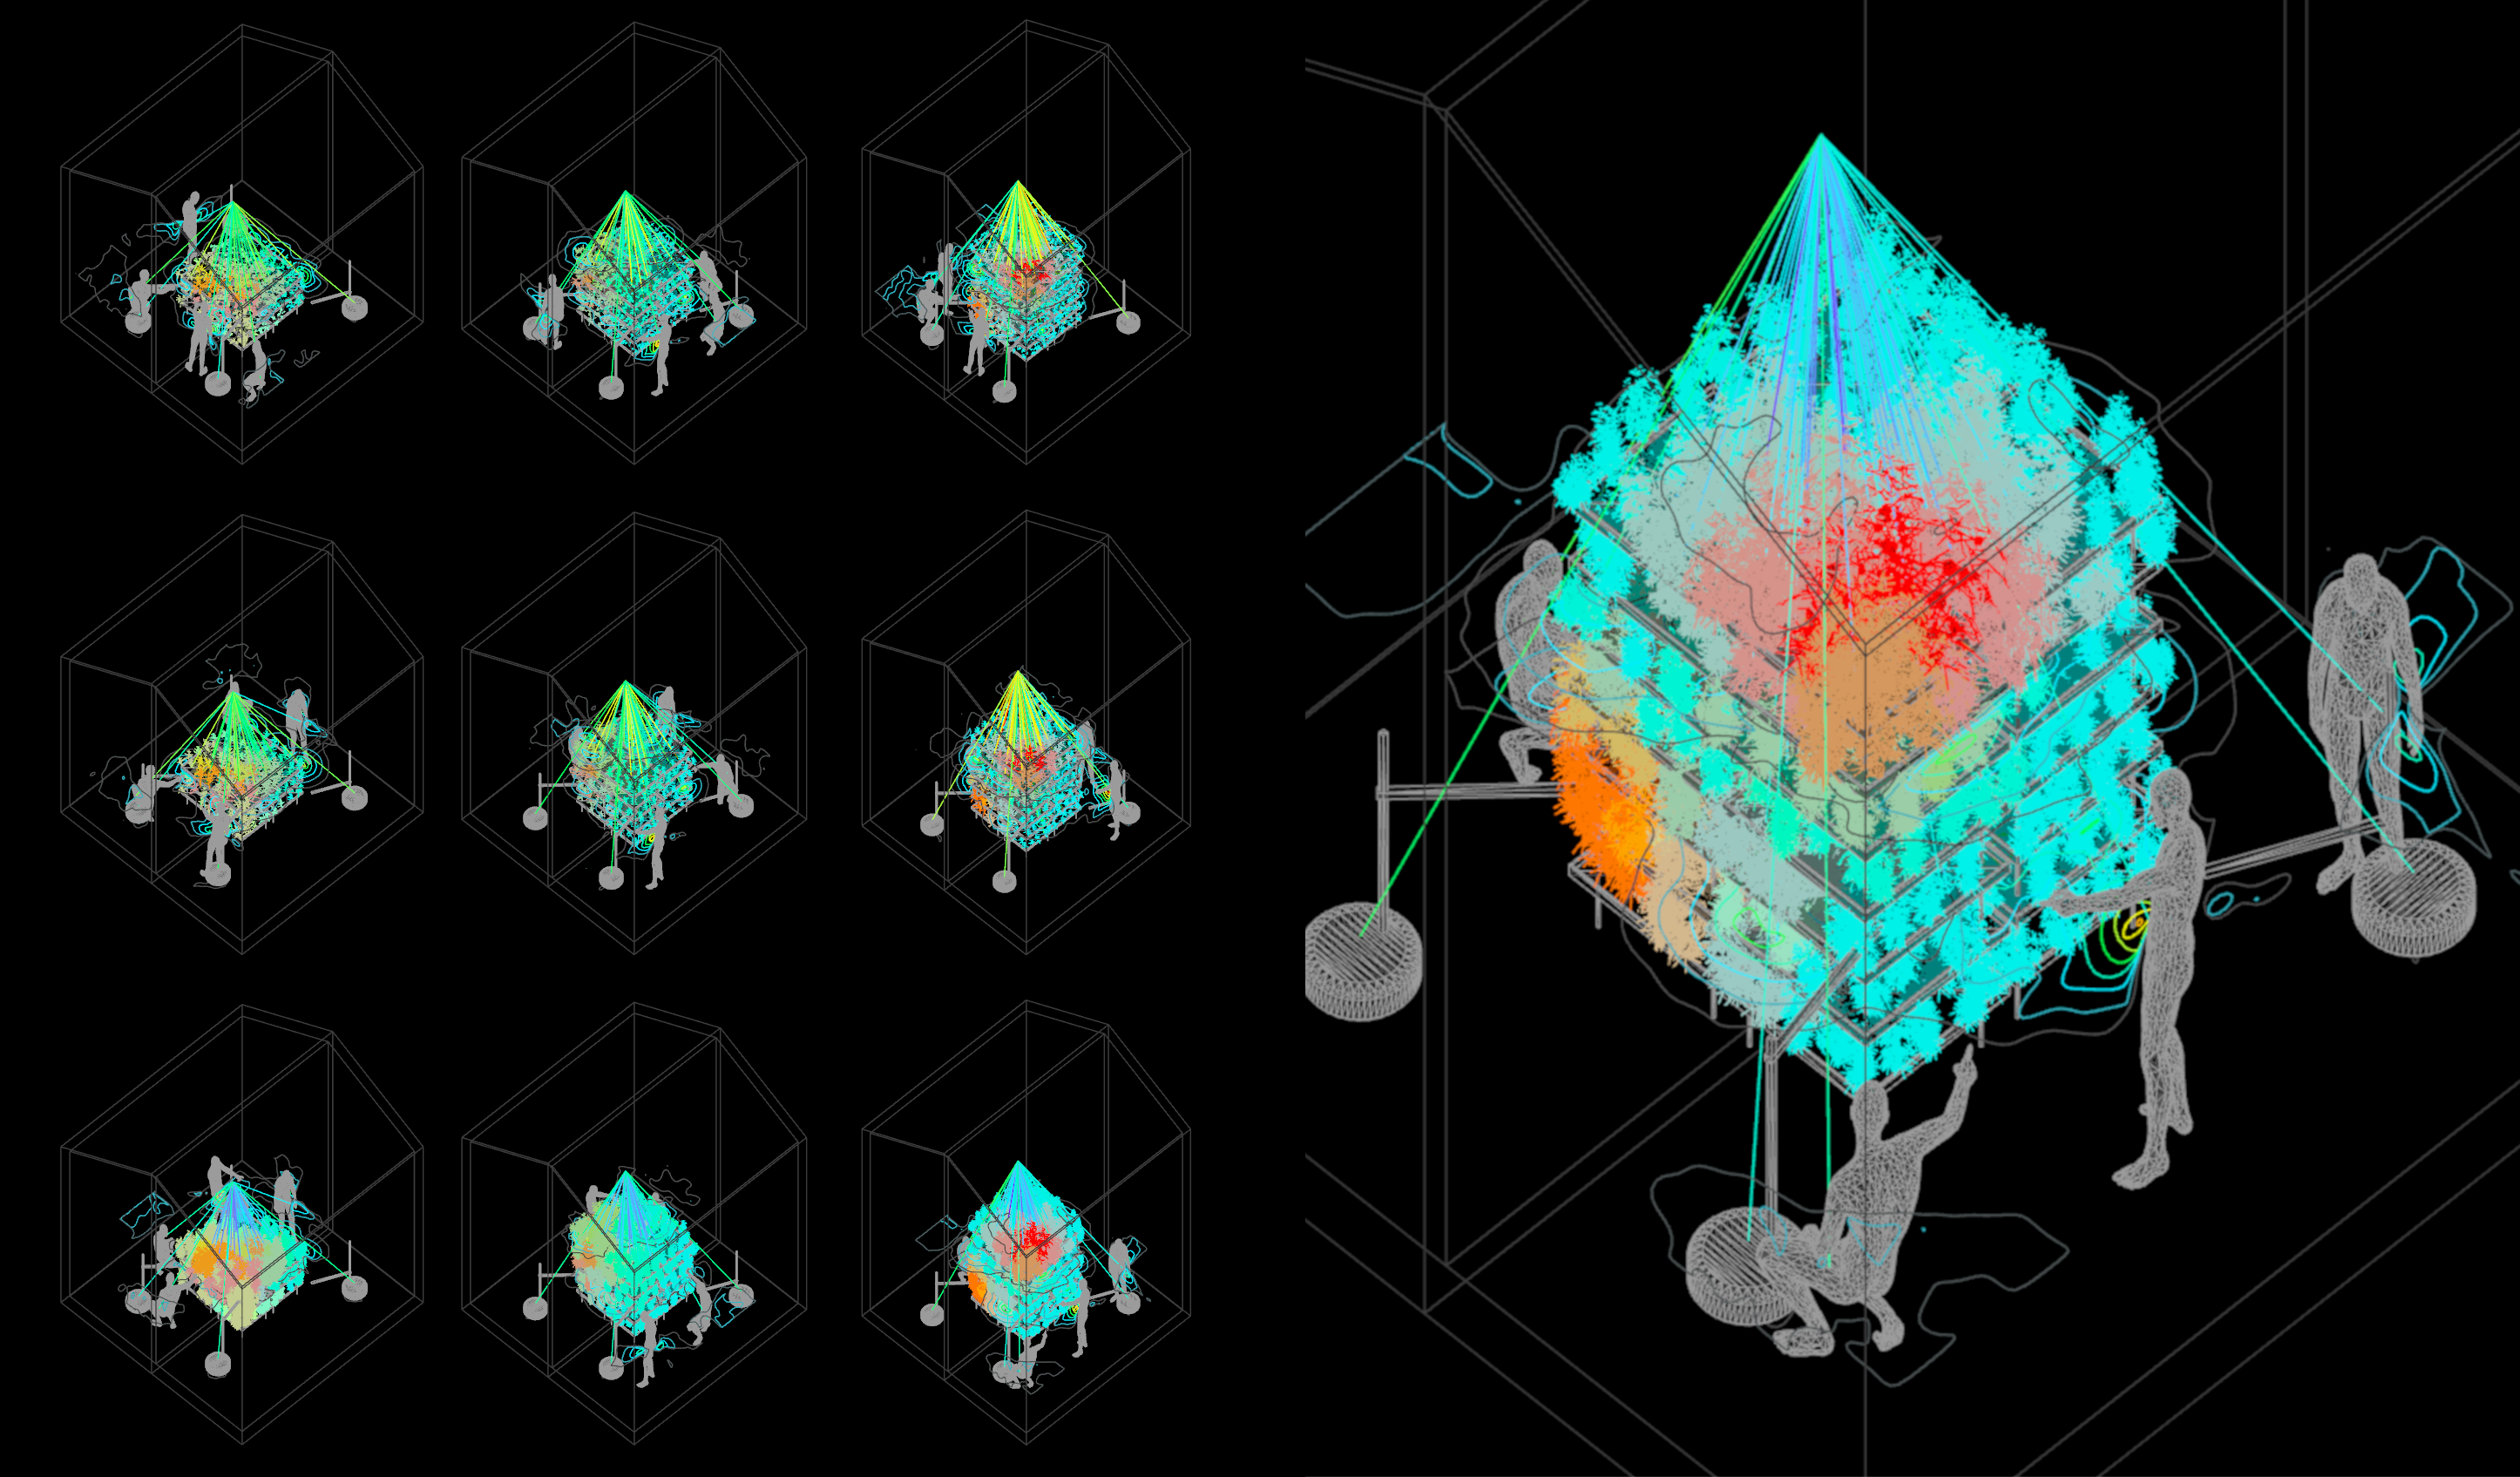
\includegraphics[width=0.98\linewidth]{figures/screenshots/combined3.png}%
    \caption{Procedurally generated cultivation scenes in Houdini, with plants on trays, infrastructure, people, robots, and devices, and the traced paths.}
    \label{fig:scene-example}
\end{figure}

% \begin{figure*}[ht]
\centering
\newcommand{\icon}[1]{\includegraphics[height=7mm]{figures/icons/#1.pdf}}
% Tools (ColorBrewer Dark2, print friendly)
\definecolor{houdini}{HTML}{D95F02}\definecolor{sionna}{HTML}{1B9E77}\definecolor{browser}{HTML}{7570B3}\definecolor{analysis}{HTML}{A6761D}
\begin{tikzpicture}[
  font=\scriptsize,
  node/.style={draw=black!75,fill=white,rounded corners=1pt,align=center,text width=2.3cm,
              minimum height=1.85cm,inner sep=2pt,line width=0.5pt,
              execute at begin node={\hyphenpenalty=10000\exhyphenpenalty=10000}},
  % A step: a white box with a bar in the colour of the tool that performs it
  step/.style={node,path picture={\fill[#1] (path picture bounding box.north west)
              rectangle ([yshift=-2.2pt]path picture bounding box.north east);}},
  output/.style={node,rounded corners=0pt},
  todo/.style={node,draw=black!50,dash pattern=on 2pt off 1.5pt},
  arr/.style={-{Latex[length=1.6mm,width=1.2mm]},line width=0.5pt,black!85},
  todoarr/.style={arr,dash pattern=on 2pt off 1.5pt},
  dot/.style={circle,fill=black!85,inner sep=0pt,minimum size=1.1mm},
  stage/.style={fill=black!7,rounded corners=2pt},
  stagelabel/.style={font=\scriptsize\bfseries,anchor=north west,inner sep=4pt,align=left},
  legend/.style={draw=black!75,fill=white,line width=0.5pt,minimum width=3.4mm,minimum height=2.6mm,inner sep=0pt},
  % The whole box links to the section that describes it.
  link/.style={alias=linked,append after command={
    let \p1=(linked.north west),\p2=(linked.south east),\n1={\x2-\x1},\n2={\y1-\y2} in
    node[inner sep=0pt,outer sep=0pt,anchor=north west] at (\p1)
      {\hyperref[#1]{\phantom{\rule{\n1}{\n2}}}}}},
]
% Stages. The boundaries run through the middle of "Check and export" (1|2) and "Results" (2|3),
% the steps that hand over from one stage to the next.
\fill[stage] (-1.35,1.95) rectangle (2.88,-4.0);
\fill[stage] (3.02,1.95)  rectangle (8.78,-1.25);
\fill[stage] (8.92,1.95) -- (13.2,1.95) -- (13.2,-4.0) -- (7.5,-4.0) -- (7.5,-1.39) -- (8.92,-1.39) -- cycle;
\node[stagelabel,link=sec:procedural] at (-1.35,1.95) {1\enspace Procedural scene generation};
\node[stagelabel,link=sec:raytracing] at (3.02,1.95)  {2\enspace Ray tracing};
\node[stagelabel,link=sec:evaluation] at (8.92,1.95)  {3\enspace Evaluation};

% 1 Procedural scene generation
\node[step=houdini,link=sec:geometry] (proc) at (0,0)
  {\icon{scene}\\[2pt]\textbf{Procedural scene}\\crops, greenhouse, devices};
\node[todo,link=sec:twin] (cal) at (0,-2.9)
  {\icon{calibrate}\\[2pt]\textbf{Calibrate}\\materials and antennas};
% 1|2 and 2 Ray tracing
\node[step=houdini,link=sec:scene] (exp) at (2.95,0)
  {\icon{export}\\[2pt]\textbf{Check and export}\\geometry and materials};
\node[step=sionna,link=sec:execution] (rt) at (5.9,0)
  {\icon{raytrace}\\[2pt]\textbf{Ray tracing}\\ on a GPU or CPU (LLVM backend), local or remote and in batches};
% 2|3 and 3 Evaluation
\node[output,link=sec:returned] (out) at (8.85,0)
  {\icon{results}\\[2pt]\textbf{Results}\\paths, links, radio maps};
\node[step=browser,link=sec:inspection] (view) at (11.8,0)
  {\icon{viewer}\\[2pt]\textbf{Web viewer}\\explore scenes, paths and maps};
\node[step=analysis,link=sec:metrics] (eng) at (8.85,-2.9)
  {\icon{engine}\\[2pt]\textbf{Application engine}\\coverage and RF energy metrics};
\node[step=houdini,link=sec:inspection] (hou) at (11.8,-2.9)
  {\icon{houdini}\\[2pt]\textbf{Inspect in Houdini}\\results on the scene};
% Towards a digital twin, below the ray-tracing stage
\node[todo,link=sec:twin] (meas) at (4.42,-2.9)
  {\icon{measure}\\[2pt]\textbf{Field measurements}\\RF and crop state};

\draw[arr] (proc)--(exp);
\draw[arr] (exp)--(rt);
\draw[arr] (rt)--(out);
\draw[arr] (out)--(view);
\draw[arr] (out.south) -- (8.85,-1.65) node[dot]{} -- (eng.north);
\draw[arr] (8.85,-1.65) -| (hou.north);
% Iteration back to the scene, around the left of the stages
\draw[arr] (view.north) -- (11.8,2.45) -- node[above,inner sep=2pt]
  {\raisebox{\dimexpr 0.55ex-1.1mm\relax}{
\includegraphics[height=2.2mm]{figures/icons/iterate.pdf}}\enspace\textit{iterate: change the scene or sweep parameters}}
  (-1.65,2.45) -- (-1.65,0) -- (proc.west);
% Field measurements are compared with the predictions and calibrate the scene
\draw[todoarr] (meas) -- node[above,inner sep=2pt]{\textit{compare}} (eng);
\draw[todoarr] (meas) -- node[above,inner sep=2pt]{\textit{calibrate}} (cal);
\draw[todoarr] (cal) -- node[left,inner sep=2pt]{\textit{update}} (proc);

% Legend: the tool behind each step
\node[anchor=north west,inner sep=0pt,align=left] at (13.5,1.95) {\textbf{Tool}\\[3pt]
  \tikz\node[legend,path picture={\fill[houdini] (path picture bounding box.north west) rectangle ([yshift=-1.4pt]path picture bounding box.north east);}]{};\enspace Houdini\\[3pt]
  \tikz\node[legend,path picture={\fill[sionna] (path picture bounding box.north west) rectangle ([yshift=-1.4pt]path picture bounding box.north east);}]{};\enspace Sionna RT\\[3pt]
  \tikz\node[legend,path picture={\fill[browser] (path picture bounding box.north west) rectangle ([yshift=-1.4pt]path picture bounding box.north east);}]{};\enspace Browser\\[3pt]
  \tikz\node[legend,path picture={\fill[analysis] (path picture bounding box.north west) rectangle ([yshift=-1.4pt]path picture bounding box.north east);}]{};\enspace Python or other\\[6pt]
  \tikz\node[legend]{};\enspace output data\\[3pt]
  \tikz\node[legend,draw=black!50,dash pattern=on 1.2pt off 0.9pt]{};\enspace not yet implemented};
\end{tikzpicture}
\caption{The \housionna{} workflow in three stages. \emph{Check and export} and \emph{Results} hand over between stages; the bar on each step shows the tool that performs it, and the square box is output data. Dashed elements are needed for an agricultural digital twin, in which field measurements calibrate the materials and antennas of the scene. Each box and stage title links to the section that describes it.}
\label{fig:pipeline}
\end{figure*}


\begin{figure*}[t]
\centering
\newcommand{\icon}[1]{\includegraphics[height=6mm]{figures/icons/#1.pdf}}
\newcommand{\card}[4][sub]{\vspace*{1.5pt}\icon{#2}\\[5pt]\textbf{#3}\\[0.5pt]{\fontsize{6.3}{7.5}\selectfont\color{#1}#4\par}}
\newcommand{\cardw}{2.45cm}\newcommand{\cardh}{1.82cm}
% Tools (jet hues as in the ray-tracing renders)
\definecolor{houdini}{HTML}{FF5A1F}\definecolor{sionna}{HTML}{76B900}\definecolor{browser}{HTML}{6A5BFF}\definecolor{analysis}{HTML}{EBCB00}
\definecolor{ink}{HTML}{000000}\definecolor{sub}{HTML}{595959}\definecolor{frame}{HTML}{A6A6A6}\definecolor{dim}{HTML}{8C8C8C}\definecolor{subdim}{HTML}{B3B3B3}\definecolor{panel}{HTML}{F0F0F0}
\begin{tikzpicture}[
  font=\fontfamily{phv}\selectfont\scriptsize,color=ink,
  every node/.append style={outer sep=0pt},
  card/.style={fill=white,draw=ink,line width=0.4pt,text=ink,inner sep=3pt,
               execute at begin node={\begin{minipage}[c][\cardh][t]{\cardw}\centering
                 \hyphenpenalty=10000\exhyphenpenalty=10000},
               execute at end node={\end{minipage}}},
  % A step: a card with a bar in the colour of the tool that performs it
  bar/.style={path picture={\fill[#1] (path picture bounding box.north west)
               rectangle ([yshift=-2.8pt]path picture bounding box.north east);}},
  step/.style={card,bar=#1},
  output/.style={card},
  % Not yet implemented: only the dashed border marks it, text and icon stay readable
  todo/.style={card,draw=dim,dash pattern=on 2pt off 1.5pt},
  arr/.style={-{Latex[length=1.5mm,width=1.1mm]},line width=0.45pt,ink,shorten >=1.5pt,shorten <=1.5pt},
  todoarr/.style={arr,dim,dash pattern=on 2pt off 1.5pt},
  lbl/.style={font=\fontfamily{phv}\selectfont\scriptsize\itshape,inner sep=2.5pt},
  % Stages are borderless panels, so arrows between stages cross no lines
  stage/.style={fill=panel},
  stagelabel/.style={font=\fontfamily{phv}\selectfont\scriptsize\bfseries,anchor=north west,inner xsep=0.2cm,inner ysep=4pt,align=left},
  num/.style={fill=black,text=white,font=\fontfamily{phv}\selectfont\tiny\bfseries,minimum size=3.2mm,inner sep=0pt},
  swatch/.style={fill=white,draw=ink,line width=0.4pt,minimum width=3.6mm,minimum height=2.6mm,inner sep=0pt},
  % The whole box links to the section that describes it.
  link/.style={alias=linked,append after command={
    let \p1=(linked.north west),\p2=(linked.south east),\n1={\x2-\x1},\n2={\y1-\y2} in
    node[inner sep=0pt,outer sep=0pt,anchor=north west] at (\p1)
      {\hyperref[#1]{\phantom{\rule{\n1}{\n2}}}}}},
]
% Grid: cards 2.66 cm wide, 0.2 cm inside each stage panel, 0.55 cm apart within a stage.
% Columns at x = 1.53, 4.74 | 8.25 | 12.41, 15.62; rows at y = 0 and -3. Every card lies inside one stage;
% the wider gap before stage 3 leaves room for the "compare" label.
\fill[stage] (0,1.6)     rectangle (6.27,-4.22);   % 1: scene and export (Houdini)
\fill[stage] (6.72,1.6)  rectangle (9.78,-1.22);   % 2: ray tracing only, top row
\fill[stage] (10.88,1.6) rectangle (17.15,-4.22);  % 3: results and their use

\node[stagelabel,link=sec:procedural] at (0,1.6)     {\tikz[baseline=(n.base)]\node[num](n){1};\enspace Procedural scene generation};
\node[stagelabel,link=sec:raytracing] at (6.72,1.6)  {\tikz[baseline=(n.base)]\node[num](n){2};\enspace Ray tracing};
\node[stagelabel,link=sec:evaluation] at (10.88,1.6) {\tikz[baseline=(n.base)]\node[num](n){3};\enspace Evaluation};

% 1 Procedural scene generation
\node[step=houdini,link=sec:geometry] (proc) at (1.53,0)  {\card{scene}{Procedural scene}{crops, greenhouse\\and devices}};
\node[step=houdini,link=sec:scene]    (exp)  at (4.74,0)  {\card{export}{Check and export}{geometry and materials}};
\node[todo,link=sec:twin]             (cal)  at (1.53,-3) {\card{calibrate}{Calibrate}{materials and antennas}};
% 2 Ray tracing
\node[step=sionna,link=sec:execution] (rt)   at (8.25,0)  {\card{raytrace}{Ray tracing}{GPU/CPU execution,\\local, remote, batched}};
% 3 Evaluation
\node[output,link=sec:returned]         (out)  at (12.41,0)  {\card{results}{Results}{paths, links, radio maps}};
\node[step=browser,link=sec:inspection] (view) at (15.62,0)  {\card{viewer}{Web viewer}{explore scenes,\\paths and maps}};
\node[step=analysis,link=sec:metrics]   (eng)  at (12.41,-3) {\card{engine}{Application engine}{coverage and\\RF energy metrics}};
\node[step=houdini,link=sec:inspection] (hou)  at (15.62,-3) {\card{houdini}{Inspect in Houdini}{results on the scene}};
% Towards a digital twin: outside the stages, below ray tracing
\node[todo,link=sec:twin]               (meas) at (8.25,-3)  {\card{measure}{Field measurements}{RF and crop state}};

\draw[arr] (proc)--(exp);
\draw[arr] (exp)--(rt);
\draw[arr] (rt)--(out);
\draw[arr] (out)--(view);
% Results feed both the application engine and Houdini: two arrows, no junction
\draw[arr] (out.south) -- (eng.north);
\draw[arr] ([xshift=5mm]out.south) |- (15.62,-1.5) -- (hou.north);

% Iteration back to the scene, from the top of the evaluation stage
\draw[arr] (14.015,1.6) -- (14.015,2.1)
  -- node[lbl,above]{\raisebox{\dimexpr 0.55ex-1.2mm\relax}{
\includegraphics[height=2.4mm]{figures/icons/iterate.pdf}}\enspace iterate: change the scene or sweep parameters}
  (-0.4,2.1) -- (-0.4,0) -- (proc.west);

% Field measurements: compared with the predictions, then calibrate the scene
\draw[todoarr] (meas) -- node[lbl,above,ink,pos=0.42]{compare} (eng);
\draw[todoarr] (meas) -- node[lbl,above,ink,pos=0.62]{calibrate} (cal);
\draw[todoarr] (cal) -- node[lbl,left,ink]{update} (proc);

% Legend: tools | output and status
\node[anchor=north,inner sep=0pt] at (8.375,-4.5) {\textbf{Tool}\quad
  \raisebox{-0.35mm}{\tikz\node[swatch,bar=houdini]{};}\enspace Houdini\quad
  \raisebox{-0.35mm}{\tikz\node[swatch,bar=sionna]{};}\enspace Sionna RT\quad
  \raisebox{-0.35mm}{\tikz\node[swatch,bar=browser]{};}\enspace Browser\quad
  \raisebox{-0.35mm}{\tikz\node[swatch,bar=analysis]{};}\enspace Python or other
  \qquad\textcolor{frame}{\rule[-0.5mm]{0.4pt}{3.5mm}}\qquad
  \raisebox{-0.35mm}{\tikz\node[swatch]{};}\enspace Output data\quad
  \raisebox{-0.35mm}{\tikz\node[swatch,draw=dim,dash pattern=on 1.2pt off 0.9pt]{};}\enspace Not yet implemented};
\end{tikzpicture}
\caption{The \housionna{} workflow in three stages. The bar on each step shows the tool that performs it; the box without a bar is output data. Dashed elements are needed for an agricultural digital twin, in which field measurements calibrate the materials and antennas of the scene. Each box and stage title links to the section that describes it.}
\label{fig:pipeline}
\end{figure*}


These applications impose different RF requirements. Active telemetry needs sufficient link margin, and batteryless operation also requires enough harvested energy per observation. Backscatter reduces the need for a sensor node to generate its own carrier~\cite{liu2013}, but requires both illumination and a return link to the gateway. Distributed \gls{wpt} depends on spatial channels and coherent combining~\cite{callebaut2024}. The propagation channel can also provide observations of the environment, as illustrated by radio tomography~\cite{wilson2010}; relating channel changes to crop conditions requires crop-specific models and independent reference measurements.

The cultivation environment affects all these links. Leaves, stems, growing trays, support structures, and greenhouse surfaces alter line-of-sight visibility and multipath. Growth changes the geometry, while water content changes the electromagnetic properties of plant tissue. Measurements in a tomato greenhouse show substantial differences from conventional propagation models~\cite{cama2019}. Deployment analysis therefore needs site-specific channels and should account for changes in the crop, device positions, and infrastructure.

Parameterised models can vary species, growth stage, spacing, leaf water content, room layout, occupancy, gateway density, and device placement without rebuilding each scene. Controlled sweeps then change selected properties while the others stay fixed, exposing placements that work for one crop configuration but fail as the canopy develops.
   

Existing workflows also address scene preparation and integration with Sionna RT. SionnaRT-Bridge connects Blender scene preparation, radio-material assignment, transmitter and receiver configuration, Sionna RT simulation, and result visualisation~\cite{ribas2026sionnartbridge}. SceneBaker generates Sionna RT-ready scenes programmatically from map and terrain data~\cite{lyu2026scenebaker}. Neither generates crop geometry or sweeps crop growth.

This paper presents \housionna{}, a workflow connecting procedural scene generation in Houdini with GPU-accelerated radio ray tracing in Sionna RT~\cite{housionna}. Its contribution is the combination of parameterised agricultural geometry, controlled crop and infrastructure sweeps, and analysis of sensor coverage and RF energy harvesting. The workflow integrates scene preparation and export, batch execution, run provenance, and inspection of paths, link metrics, and radio maps in Houdini or a web viewer; Sionna RT provides the electromagnetic solver~\cite{hoydis2023,aoudia2025}. A batteryless plant-sensor use case brings these stages together to examine connectivity, charge time, and the choice of harvester.

\Cref{fig:pipeline} outlines the workflow, and \cref{fig:scene-example} shows example scenes. \Cref{sec:procedural,sec:raytracing,sec:evaluation} describe procedural scene generation, ray tracing, and evaluation, respectively. \Cref{sec:casestudy} applies the workflow to the plant-sensor use case, and \cref{sec:conclusion} discusses limitations and the steps towards an agricultural digital twin.


